\documentclass[11pt,a4paper]{article}
\usepackage[utf8]{inputenc}
\usepackage[T1]{fontenc}
\usepackage[margin=2.5cm]{geometry}
\usepackage{amsmath}
\usepackage{booktabs}
\usepackage{graphicx}
\usepackage{enumitem}
\usepackage[hidelinks]{hyperref}

\usepackage{xurl}
\makeatletter\g@addto@macro\UrlBreaks{\do\_}\makeatother
\newcommand{\code}[1]{\path{#1}}
\sloppy

\title{Kanizsa saliences: project report and current status}
\author{Francesco Mannella}
\date{October 1, 2026 \\ \small branch \code{saliencies}, commit \code{69f2588} plus uncommitted changes}

\begin{document}
\maketitle
\tableofcontents

\section{Summary}

The project simulates an eye that explores a simple coloured object (a triangle
or a square) and learns, without supervision, a set of fixation goals and the
saccades that reach them. A bottom-up saliency front end moves the eye; an
\emph{offline controller} made of three aligned topological maps learns to
associate what the fovea sees before a saccade, the attention target that
drives the saccade, and what the fovea sees after it. A competence predictor
measures how well the three maps agree and gates both exploration and
plasticity. After training, the controller is tested on rotated objects and the
sequence of goals it selects (the \emph{scanpath}) is analysed.

Status in brief:
\begin{itemize}[nosep]
  \item The training pipeline, the test pipeline, the scoring scripts and a
    results web server are in place and documented in \code{SCRIPTS.md}.
  \item A hyperparameter campaign (September 26--27) settled on
    \code{anchor_std} 4 and \code{neighborhood_modulation_baseline} 0.5 as the
    reference configuration: competence about 0.73--0.78 at 1000 epochs with
    well-ordered visual maps.
  \item Test scanpaths were too short (2--3 distinct goals). Inhibition of
    recent goals lengthens them to 5--6 goals at a small cost in separation
    between objects.
  \item A tracing of the executed eye movements showed that salience-driven
    saccades undo a large share of the goal saccades. The opt-in
    \code{hold_fixation} removes them completely, but with it the scanpaths of
    different rotations share more goals and the two objects are less
    separated on the map.
  \item The latest change, \code{orienting_saccade} (uncommitted), removes the
    shared starting goal that \code{hold_fixation} introduces. Applied at test
    time to the hold-fixation controllers, it brings goal sharing back to the
    level of the runs without hold fixation (0.11--0.32 of test pairs against
    0.68--0.78). Separation between objects recovers fully without goal
    inhibition and only partly with it.
\end{itemize}

\section{Model}

\subsection{Environment}

\code{tools/EyeSim} is a Gymnasium environment (\code{EyeSim/EyeSim-v0}) built on
Box2D. The task space is $80\times80$ units and contains one coloured object
taken from \code{models/worlds.json}. An observation is a dict with
\code{RETINA}, an $80\times80\times3$ view of an $80\times80$ window centred on
the eye position, and \code{FOVEA}, its central $16\times16$ crop. The action is
a two-dimensional displacement of the eye position, clipped to the task space.
There is no reward and episodes never terminate. During training the world is
chosen per epoch (\code{epoch \% 100 < triangles_percent} gives the triangle,
otherwise the square), so each update sees a single object class. Two details
matter for the analysis of rotations: the ``square'' is a $31.7\times26.5$
rectangle, and objects rotate about the body origin, not the centroid.

\subsection{Saliency front end and agent}

\code{model/gabor_filtering.py} applies a bank of Gabor kernels to
channel-opponent versions of the retina (red against green, green against red,
blue against red and green) and to a brightness channel.
\code{model/visual_processing.py} builds the bank from the \code{gabor_*}
parameters; orientations are \code{linspace(0, 180, bins)[:-1]} degrees.

The agent (\code{model/agent.py}) takes the channel mean of the adjusted
saliency, normalizes it and multiplies it by a Gaussian attentional mask centred
on a normalized point $c$ of the retina. With retina side $W$, the mask variance
along each axis is
\[
  \sigma^2 = W\,v^2\,\bigl(f + p\,(1-\tanh(s\,\lVert c-0.5\rVert))\bigr),
\]
where $v$ is \code{attention_max_variance}, $f$ is
\code{attention_fixed_variance_prop}, $p$ is
\code{attention_center_distance_variance_prop} and $s$ is
\code{attention_center_distance_slope}. Note that $v$ enters squared, which may
be unintended. A pixel is then sampled with probability proportional to
$\max(0, a_i - \rho\max a)$, with $\rho$ = \code{agent_sampling_precision}; with
the values used in the sweeps ($\rho = 0.999999$) this is practically the
argmax. The action is the displacement that centres the retina on that pixel.

The visual input of the controller is the \emph{colour-saliency fovea}: the
colour-opponent saliency in the central \code{fovea_scale} retina pixels, resized
to \code{fovea_size} and multiplied by \code{fovea_gain}.

\subsection{Offline controller}

\code{model/offline_controller.py} holds three topological maps that share a
$10\times10$ grid (\code{maps_output_size} = 100):
\begin{itemize}[nosep]
  \item \textbf{visual conditions}: the fovea before a saccade;
  \item \textbf{visual effects}: the fovea after the saccade;
  \item \textbf{attention}: the normalized attention centre that produced it.
\end{itemize}
Each map computes the squared distance of its input from every unit's prototype.
The winner on the visual-conditions map is the \emph{goal}.

\paragraph{Learning.} The maps are trained with a supervised-topological-map
(STM) loss. For a sample with squared distances $d_j^2$ to the units,
\[
  L = \tfrac{1}{2}\sum_j d_j^2\,\phi_j\,\psi_j ,
\]
where $\phi$ is a Gaussian neighbourhood around the map's own winner and $\psi$
a Gaussian of width \code{anchor_std} around the goal. The anchor is what aligns
the three maps: the attention and visual-effects prototypes for a saccade are
pulled to the grid location of the goal. Updates use Adam.

\paragraph{Competence.} For each sample the \emph{match} is the mean, over the
attention and visual-effects winners, of $\exp(-(d/\sigma_m)^2)$, with $d$ the
grid distance from the goal and $\sigma_m$ = \code{match_std}. A logistic
predictor (\code{model/predict.py}) is trained to output the match from a
Gaussian bump on the goal. Its output, rescaled from $[0.5,1]$ to $[0,1]$, is
the local competence of a goal; its mean over all units is the global
competence $C$.

\paragraph{Competence-based modulation.} With
$I = 1-\tanh(\texttt{decaying\_speed}\cdot C)$ and a per-sample
$I_\ell = 1-\tanh(\texttt{local\_decaying\_speed}\cdot c_\ell)$, both the
neighbourhood width and the loss weight are
$\text{baseline} + \text{gain}\cdot I\cdot I_\ell$. Because Adam normalizes the
gradient scale, the loss weight does not actually shrink the steps; the opt-in
\code{maps_lr_decay} lowers the Adam learning rate directly.

\paragraph{Choosing a saccade.} Given a fovea, the controller finds the goal and
its local competence $c$. With probability $c$ it returns the attention-map
prototype at the goal; otherwise it returns a random attention centre (on a ring
at distance 0.3--0.6 from the retina centre, or uniform in $[0.1,0.9]^2$ with
\code{random_saccade='uniform'}). Exploration therefore fades as competence
grows.

\subsection{Training loop}

\code{src/main.py}; see also \code{pseudocode.md}. An epoch is \code{episodes}
$\times$ \code{saccade_num} $\times$ \code{saccade_time} steps
($20\times10\times10$ in the sweeps). Within each saccade:
\begin{enumerate}[nosep]
  \item at the midpoint step the controller proposes an attention centre from
    the current fovea and the agent's mask is set there;
  \item on the other steps the mask is reset to the retina centre;
  \item at every step the agent samples a salient point under the mask and the
    eye moves there;
  \item fovea, action, attention centre and competence are recorded.
\end{enumerate}
At the end of the epoch the steps whose action norm exceeds
\code{saccade_threshold} are kept. For each one, the fovea two steps before is
the visual condition, and the fovea and attention two steps after are the
effect and the action. The three maps and the predictor are then updated, and
the controller is saved to \code{off_control_store}, from which training can
resume.

\subsection{Test and generative extension}

\code{src/test.py} runs one episode on a chosen object, position and rotation.
At each decision the goal's attention prototype is always used (no exploration),
and the sequence of goals is saved to \code{goals-<world>-<pos>-<rot>.npy}.
\code{scripts/tests.py} runs it for both objects at rotations 0.0--1.6 rad in
steps of 0.2.

\code{src/test_generative.py} adds a FORCE-trained reservoir
(\code{model/recurrent_generative_model.py}) that encodes the sequence of goals
and predicts the next one; its prediction filters the visual-conditions map, and
an occluder can be placed on the object. No script in the repository trains the
reservoir (\code{rnn_store.npy} must come from elsewhere), so this branch is
currently not usable end to end.

\section{Tooling}

All scripts are described in \code{SCRIPTS.md}. The main ones:

\begin{center}
\begin{tabular}{@{}p{4.6cm}p{10.4cm}@{}}
\toprule
Script & Purpose \\
\midrule
\code{scripts/grid_search.py} & trains a grid, or a base configuration plus named one-factor variants, over several seeds \\
\code{scripts/tests.py} & runs the test scanpaths on every run of a sweep; resumes interrupted folders \\
\code{scripts/evaluate_runs.py} & ranks runs on competence, weight stability, topography and prototype definition \\
\code{scripts/ls_sims.py}, \code{score_folder.py}, \code{chain_*.py} & scanpath scores from the goals files \\
\code{scripts/results_server.py} & web page per run: curves, maps, test animations, scanpath tiles (object region purity, symmetry-aware goal sharing) \\
\code{src/local_wandb.py} & local stand-in for wandb; runs log to \code{data_sim/} unless \code{-w} \\
\bottomrule
\end{tabular}
\end{center}

All sweeps live in named folders under \code{tests/} (a symlink to
\code{/home/fmannella/tmp/kanizsa_saliences}); the original runs are in
\code{tests/old/}.

\section{Development history}

\begin{itemize}[nosep]
  \item \textbf{Early work (branch history up to \code{beb4147}).} Environment
    in degrees and then in task-space units, Gabor saliency, colour saliency,
    attentional mask, refactoring of agent and main, pseudocode.
  \item \textbf{Tooling port and audit (\code{138788a}--\code{a80fb6b}).} The
    analysis and orchestration tools of \code{main} were ported, the scripts
    documented and thirteen issues (S1--S13) fixed. Several fixes change the
    results with respect to the old runs; the main ones are listed in
    Section~\ref{sec:compat}.
  \item \textbf{Infrastructure (\code{5880598}--\code{ff4f87d}).} Results web
    server, local logging, a roughly sixfold speed-up with bit-identical
    results.
  \item \textbf{Evaluation and opt-in switches (\code{642f129} onwards).}
    Run evaluation, one-factor sweeps, \code{maps_lr_decay},
    \code{random_saccade}, \code{goal_inhibition}, \code{hold_fixation}, and
    (uncommitted) \code{orienting_saccade}. Every switch defaults to the
    previous behaviour.
\end{itemize}

\subsection{Changes that break comparison with earlier runs}
\label{sec:compat}

\begin{itemize}[nosep]
  \item The competence predictor is trained on each sample's own match; a shape
    bug used to train every sample towards the batch mean.
  \item The match no longer has a constant third term that put a floor of 1/3
    under it.
  \item Training and both test scripts now query the maps with the
    colour-saliency fovea, the same input the maps are trained on. The
    \code{long_search} runs are therefore not reproducible with current code.
  \item Gabor orientations cover the half circle instead of the full circle.
  \item \code{epochs} is the total number of epochs on resume;
    \code{--posrot} angles are in radians as given; \code{paths.csv} drops the
    first three saccades of each test.
\end{itemize}

\section{Experiments and results}

The base configuration of every sweep is that of
\code{long_search_b71233_090902} (\code{match_std} 10, \code{anchor_std} 2,
\code{neighborhood_modulation} 40 with baseline 0.1,
\code{learningrate_modulation} 50, \code{local_decaying_speed} 0.5,
\code{maps_learning_rate} 0.1). Runs are deterministic given parameters and
seed: the base at 1000 epochs reproduces the replay of the original run exactly.

\subsection{Map quality and competence (September 26--27)}

Runs are scored by \code{scripts/evaluate_runs.py}: competence over the last 20
epochs; Spearman correlation between grid and prototype distances and
topographic error for topography; dead units and prototype contrast for
definition; relative weight change for stability.

\paragraph{Screening and refinement (300 and 500 epochs).} Among twelve
single-factor changes, \code{anchor_std} 4 was the most useful. At 500 epochs
over three seeds it gave Spearman 0.93 against 0.81 on the visual-conditions
map and 0.87 against 0.69 on the visual-effects map, with equal competence
(0.63 against 0.62). Low constant learning rates (0.01, 0.03) prevented
prototypes from forming; \code{match_std} 6 only lowered the competence scale;
\code{maps_lr_decay} improved the attention map and stability but capped
competence (0.46 with decay 0.5).

\paragraph{Long training (1000 epochs).} Table~\ref{tab:maps} gives the means
over three seeds. With \code{anchor_std} 4 the maps stay better ordered than
the base but competence is lower; raising the neighbourhood baseline to 0.5
recovers the competence and keeps the topography. A fourth round found no gain
from a baseline of 0.8 or from uniform exploration.

\begin{table}[h]
\centering\small
\begin{tabular}{@{}lccccc@{}}
\toprule
Configuration & Competence & Spearman vc & Spearman att & Topo.\ err.\ att & Dead att \\
\midrule
base (anchor 2, baseline 0.1) & $0.772\pm0.019$ & 0.78 & 0.46 & 0.39 & 0.64 \\
anchor 3                      & $0.760\pm0.023$ & 0.79 & 0.51 & 0.26 & 0.54 \\
anchor 4                      & $0.735\pm0.033$ & 0.88 & 0.53 & 0.11 & 0.44 \\
anchor 4, baseline 0.3        & $0.741\pm0.029$ & 0.88 & 0.58 & 0.12 & 0.48 \\
anchor 4, baseline 0.5        & $0.778\pm0.011$ & 0.89 & 0.55 & 0.07 & 0.47 \\
\bottomrule
\end{tabular}
\caption{Map quality at 1000 epochs, three seeds. vc: visual-conditions map;
att: attention map. Dead: share of units that never win.}
\label{tab:maps}
\end{table}

\paragraph{Seed variance.} With five seeds the advantage of baseline 0.5 is less
clear-cut: competence $0.727\pm0.063$ for 0.5, $0.747\pm0.054$ for 0.65 and
$0.733\pm0.028$ for 0.8. The differences between these three baselines are
within the seed spread. \code{anchor_std} 4 with baseline 0.5 was kept as the
reference for all later work.

\begin{figure}[h]
\centering
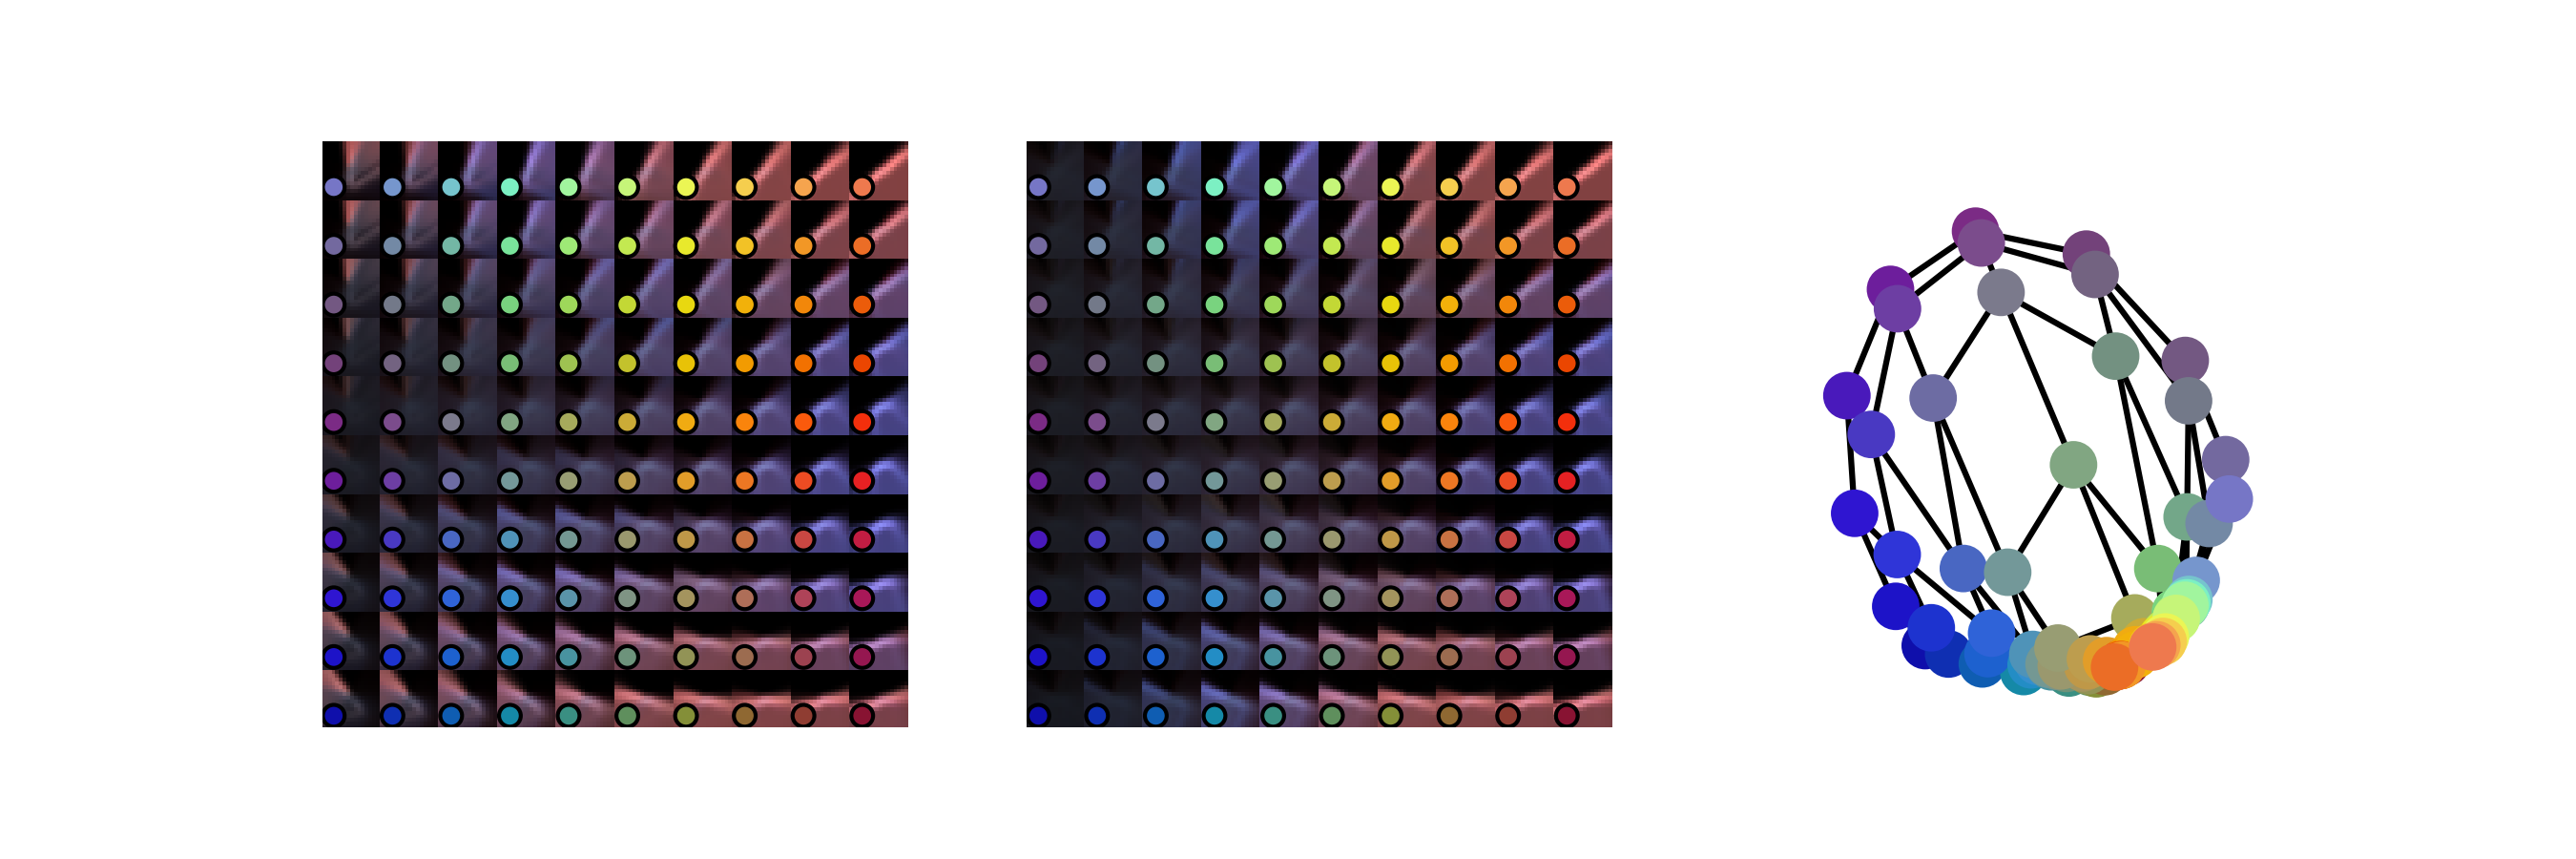
\includegraphics[width=\textwidth]{figures/maps_anchor4_nmb05.png}
\caption{Maps after 1000 epochs for the reference configuration, seed 93581.
Left and centre: prototypes of the visual-conditions and visual-effects maps on
the $10\times10$ grid. Right: the attention map's prototypes in retina
coordinates, linked by grid adjacency.}
\end{figure}

\paragraph{Open point.} The attention map remains the weakest: almost half of
its units never win, and its topography erodes between 500 and 1000 epochs
(Spearman 0.65 to 0.53 for anchor 4).

\subsection{Scanpath criteria}

A good set of test scanpaths, as agreed on September 28, satisfies two
conditions on the visual-conditions grid:
\begin{enumerate}[nosep]
  \item the goals of all rotations of one object stay in a region separate from
    the other object's;
  \item scanpaths of different rotations share no goals, since each rotation is
    a different shape. Rotations equivalent under the object's symmetry
    (90$^\circ$ for the square, 120$^\circ$ for the triangle, within 0.1 rad)
    are excluded from this penalty.
\end{enumerate}
The measures used below are: \emph{kNN purity} (share of goals whose nearest
goal from another test belongs to the same object), \emph{pairs sharing} (share
of test pairs with at least one goal in common) and the mean number of distinct
\emph{goals} per test.

\begin{figure}[h]
\centering
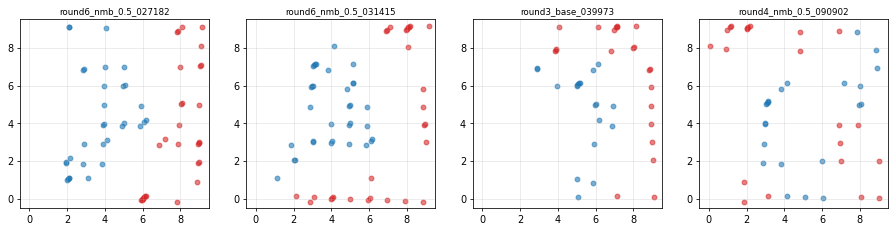
\includegraphics[width=\textwidth]{figures/region_examples.png}
\caption{Goals of all test scanpaths on the visual-conditions grid for four
runs; the two colours are the two objects.}
\end{figure}

On the runs of the previous section the objects were already well separated
(purity 0.92--0.99) but each test visited only 2.3--2.9 distinct goals: the
scanpath locks onto one goal or oscillates between two.

\subsection{Inhibition of recent goals (September 28--29)}

\code{goal_inhibition} multiplies the visual-conditions distances by
$1 + s\,g$, where $g$ is a Gaussian bump on the grid around each of the last
$m$ goals of the episode. Table~\ref{tab:ior} shows the effect of the strength
$s$ when the inhibition is used in training and in tests ($m=3$, width 1, five
seeds).

\begin{table}[h]
\centering
\begin{tabular}{@{}lcccc@{}}
\toprule
Strength $s$ & Competence & kNN purity & Pairs sharing & Goals per test \\
\midrule
0   & 0.727 & 0.958 & 0.197 & 2.80 \\
0.5 & 0.714 & 0.927 & 0.300 & 5.26 \\
1   & 0.729 & 0.926 & 0.301 & 5.56 \\
1.5 & 0.748 & 0.873 & 0.304 & 5.67 \\
2   & 0.726 & 0.881 & 0.354 & 6.29 \\
\bottomrule
\end{tabular}
\caption{Inhibition strength, trained with inhibition, 1000 epochs, five seeds.}
\label{tab:ior}
\end{table}

The inhibition roughly doubles the number of goals without changing competence.
Longer scanpaths share goals more often, and separation between objects falls
for $s\ge1.5$. Applying a strong inhibition ($s=5$) only at test time to runs
trained without it degrades separation clearly (purity 0.81, pairs sharing
0.48). Varying the memory and width (three seeds) showed that a memory of 5 or
8 lengthens the scanpaths further (about 7 goals) but lowers purity to
0.84--0.88; a narrow bump (width 0.5, memory 3) gave the best balance
(purity 0.92, pairs sharing 0.24, 5.1 goals) and became the setting for the
following sweeps.

\subsection{Salience saccades undo goal saccades (September 30)}

Goals files record only decisions. Tracing the eye movements actually executed
by the environment showed that, after each decision, the attention mask is reset
to the retina centre with a standard deviation of about 54 pixels on an
80-pixel retina. That mask is nearly flat, so the next step saccades to the
global salience maximum and frequently reverses the goal saccade. The fovea
then returns to the same view and the goal does not change. Training has the
same structure.

\begin{table}[h]
\centering
\begin{tabular}{@{}lccc@{}}
\toprule
Configuration & Goal not executed & Salience saccades & Goal reversed \\
\midrule
reference, no inhibition          & 0.108 & 0.255 & 0.426 \\
inhibition (1, 3, 0.5)            & 0.192 & 0.234 & 0.331 \\
\quad + attention variance 4      & 0.022 & 0.320 & 0.538 \\
\quad + attention variance 3      & 0.040 & 0.183 & 0.143 \\
\quad + attention variance 2      & 0.682 & 0.045 & 0.223 \\
hold fixation, no inhibition      & 0.212 & 0.000 & 0.000 \\
hold fixation + inhibition        & 0.104 & 0.000 & 0.000 \\
\quad + attention variance 3      & 0.000 & 0.000 & 0.000 \\
\bottomrule
\end{tabular}
\caption{Executed eye movements in tests (three seeds, both objects, rotations
0, 0.6 and 1.2). Goal not executed: share of decision steps without an eye
movement. Salience saccades: share of non-decision steps with one. Goal
reversed: share of goal saccades undone at the next step. Default attention
variance is 6.}
\label{tab:trace}
\end{table}

\paragraph{Narrower masks.} Lowering \code{attention_max_variance} reduces the
salience saccades but never removes them, and at 2 learning collapses
(competence 0.28, purity 0.46). Value 3 is the best compromise on the trace but
lowers competence (0.70 against 0.74) and separation.

\paragraph{Hold fixation.} \code{hold_fixation} zeroes the action on every step
except the decision step, in training and in tests, so each goal produces
exactly one saccade. It removes salience saccades and reversals entirely
(Table~\ref{tab:trace}). The scanpaths, however, get worse by the criteria above
(Table~\ref{tab:hold}): purity drops from about 0.93 to 0.84--0.86 and the share
of test pairs with a common goal rises from about 0.2 to 0.7. Map definition
also declines (visual-conditions contrast 0.74--0.79 against 0.88--0.90), while
the attention map uses more of its units.

\begin{table}[h]
\centering
\begin{tabular}{@{}lcccc@{}}
\toprule
Configuration & Competence & kNN purity & Pairs sharing & Goals per test \\
\midrule
no hold, no inhibition     & 0.778 & 0.932 & 0.173 & 2.41 \\
no hold, inhibition        & 0.738 & 0.924 & 0.237 & 5.13 \\
no hold, inhib., variance 3 & 0.696 & 0.883 & 0.340 & 5.83 \\
hold, no inhibition        & 0.710 & 0.863 & 0.675 & 3.33 \\
hold, inhibition           & 0.668 & 0.841 & 0.675 & 6.28 \\
hold, inhib., variance 3   & 0.727 & 0.862 & 0.781 & 6.41 \\
\bottomrule
\end{tabular}
\caption{Hold fixation, 1000 epochs, three seeds.}
\label{tab:hold}
\end{table}

\paragraph{Diagnosis.} With hold fixation the first decision of every episode
is taken from the initial view, in which retina and object are both at the
centre of the task space. That view is nearly the same for every rotation, so
all scanpaths start from a shared hub goal, which inflates goal sharing.

\subsection{Orienting saccade (October 1)}

\code{orienting_saccade} adds one salience saccade with a uniform mask at the
start of each episode, before the first goal decision; it is not recorded for
training. The nine hold-fixation controllers of Table~\ref{tab:hold} were
re-tested with the switch on (\code{tests/scanpath_orient_2026-10-01}); they
were trained without it.

\begin{table}[h]
\centering
\begin{tabular}{@{}lccccc@{}}
\toprule
Configuration & kNN purity & Pairs sharing & Goals per test & First goals \\
\midrule
hold, no inhibition              & 0.863 & 0.675 & 3.33 & 1.7 \\
\quad + orienting saccade        & 0.935 & 0.110 & 2.41 & 12.3 \\
hold, inhibition                 & 0.841 & 0.675 & 6.28 & 2.3 \\
\quad + orienting saccade        & 0.840 & 0.283 & 5.59 & 13.0 \\
hold, inhib., variance 3         & 0.862 & 0.781 & 6.41 & 2.0 \\
\quad + orienting saccade        & 0.880 & 0.320 & 6.13 & 10.7 \\
\bottomrule
\end{tabular}
\caption{Orienting saccade at test time on the hold-fixation controllers, three
seeds. First goals: number of distinct first goals over the 18 tests of a run
(two objects, nine rotations).}
\label{tab:orient}
\end{table}

\paragraph{Result.} The shared hub goal is gone: the 18 tests of a run start
from 10--13 different goals instead of 1--4. Goal sharing falls to the level of
the runs without hold fixation (Table~\ref{tab:hold}: 0.17 without inhibition,
0.24 with it). Without inhibition, purity is also back (0.935 against 0.932),
with the same number of goals per test (2.4), so that configuration now matches
the reference on the scanpath measures while executing every goal saccade
faithfully. With inhibition, purity does not recover (0.84, and 0.76--0.78 on
two of the three seeds), so the objects remain less separated than without
hold fixation (0.92).

\paragraph{Limits.} The switch was applied at test time only, and the executed
eye movements were not re-traced for these runs.

\section{Current status}

\subsection{Work in progress}

\code{orienting_saccade} (uncommitted; \code{src/main.py}, \code{src/test.py},
\code{src/params.py}, \code{SCRIPTS.md}) adds one salience saccade with a
uniform mask at the start of each episode, so that the first decision depends
on the rotation when \code{hold_fixation} is on. Its test-time evaluation is in
Table~\ref{tab:orient}.

\begin{itemize}[nosep]
  \item \code{tests/orient_verify_2026-10-01}: short runs comparing the
    committed code, the new code with the switch off, and the switch on.
    This report did not re-check their outcome.
  \item \code{tests/scanpath_orient_2026-10-01}: the test sweep reported
    above; complete (18 goals files for each of the nine runs).
  \item Not yet run: a sweep that trains with \code{orienting_saccade}.
\end{itemize}

\subsection{Reference configuration}

\begin{center}
\begin{tabular}{@{}ll@{}}
\toprule
Parameter & Value \\
\midrule
\code{epochs}, \code{episodes}, \code{saccade_num}, \code{saccade_time} & 1000, 20, 10, 10 \\
\code{maps_output_size}, \code{maps_learning_rate} & 100, 0.1 \\
\code{anchor_std}, \code{match_std} & 4, 10 \\
\code{neighborhood_modulation}, baseline & 40, 0.5 \\
\code{learningrate_modulation}, baseline & 50, 0.02 \\
\code{decaying_speed}, \code{local_decaying_speed} & 3, 0.5 \\
\code{saccade_threshold}, \code{agent_sampling_precision} & 12, 0.999999 \\
\code{gabor_scales}, bins, kernel size & [1.0], 5, 5 \\
\code{gabor_rgb_prop}, \code{gabor_bright_prop} & 10, 0 \\
\code{attention_max_variance}, fixed, distance, slope & 6, 0.3, 0.7, 2 \\
\code{fovea_scale}, \code{fovea_size} & [16, 16], [16, 16] \\
\code{goal_inhibition}, memory, width (when on) & 1, 3, 0.5 \\
\bottomrule
\end{tabular}
\end{center}

These are the sweep values, not the defaults of \code{src/params.py}, which
differ for several parameters (for example \code{anchor_std} 8,
\code{match_std} 4, \code{neighborhood_modulation} 10).

\subsection{Open problems}

\begin{enumerate}[nosep]
  \item \textbf{Faithful saccades against good scanpaths.} Without
    \code{hold_fixation} the recorded scanpaths look good but 33--43\% of the
    goal saccades are reversed by salience; with it the saccades are faithful
    but the scanpaths overlap. \code{orienting_saccade} closes the gap at test
    time when goal inhibition is off; with inhibition the scanpaths are longer
    but the objects stay less separated (purity 0.84 against 0.92). Training
    with the switch on has not been tried.
  \item \textbf{Attention map.} High share of dead units and late erosion of
    its topography in the configurations without hold fixation.
  \item \textbf{Mask variance.} \code{attention_max_variance} enters the
    variance squared, and \code{attention_fixed_variance_prop} does not narrow
    the reset mask. Not yet decided whether to change the formula.
  \item \textbf{Weight stability.} Weights settle with training time rather
    than through the competence modulation, since Adam cancels the loss
    scaling. \code{maps_lr_decay} works but caps competence at the values
    tried (0.2, 0.5, 0.9).
  \item \textbf{Generative model.} \code{test_generative.py} cannot be run
    without an externally produced \code{rnn_store.npy}.
  \item \textbf{Block curriculum.} The object is chosen per epoch, so each
    update sees one class. This is by design but has not been compared with
    mixed epochs.
  \item \textbf{Seed variance.} Several differences reported above are of the
    same size as the spread between seeds; most later sweeps used three seeds.
\end{enumerate}

\subsection{Repository state}

\begin{itemize}[nosep]
  \item Modified, not committed: \code{SCRIPTS.md}, \code{src/main.py},
    \code{src/params.py}, \code{src/test.py} (the \code{orienting_saccade}
    switch).
  \item Untracked: \code{knowledgebase/} (reference papers and reviews),
    \code{log}, \code{retina_poses.npy}, \code{src/model/gabor_test.png},
    \code{tests} (symlink), and this \code{docs/} folder.
  \item Unused parameters still present in \code{params.py}:
    \code{match_std_baseline}, \code{colors}, \code{magnitude_decay}.
\end{itemize}

\end{document}
